\hypertarget{dcs__driver_8c}{
\section{dcs\_\-driver.c File Reference}
\label{dcs__driver_8c}\index{dcs_driver.c@{dcs\_\-driver.c}}
}
{\tt \#include $<$linux/kernel.h$>$}\par
{\tt \#include $<$linux/init.h$>$}\par
{\tt \#include $<$asm/uaccess.h$>$}\par
{\tt \#include $<$linux/fs.h$>$}\par
{\tt \#include $<$linux/types.h$>$}\par
{\tt \#include $<$linux/sched.h$>$}\par
{\tt \#include $<$linux/errno.h$>$}\par
{\tt \#include $<$linux/slab.h$>$}\par
{\tt \#include $<$asm/io.h$>$}\par
{\tt \#include $<$linux/mm.h$>$}\par
{\tt \#include $<$linux/ioport.h$>$}\par
{\tt \#include $<$linux/spinlock.h$>$}\par
{\tt \#include $<$asm/system.h$>$}\par
{\tt \#include $<$linux/module.h$>$}\par
{\tt \#include \char`\"{}dcs\_\-driver.h\char`\"{}}\par
{\tt \#include \char`\"{}version.h\char`\"{}}\par
{\tt \#include \char`\"{}mr\-Kern\-Logging.h\char`\"{}}\par


Include dependency graph for dcs\_\-driver.c:\begin{figure}[H]
\begin{center}
\leavevmode
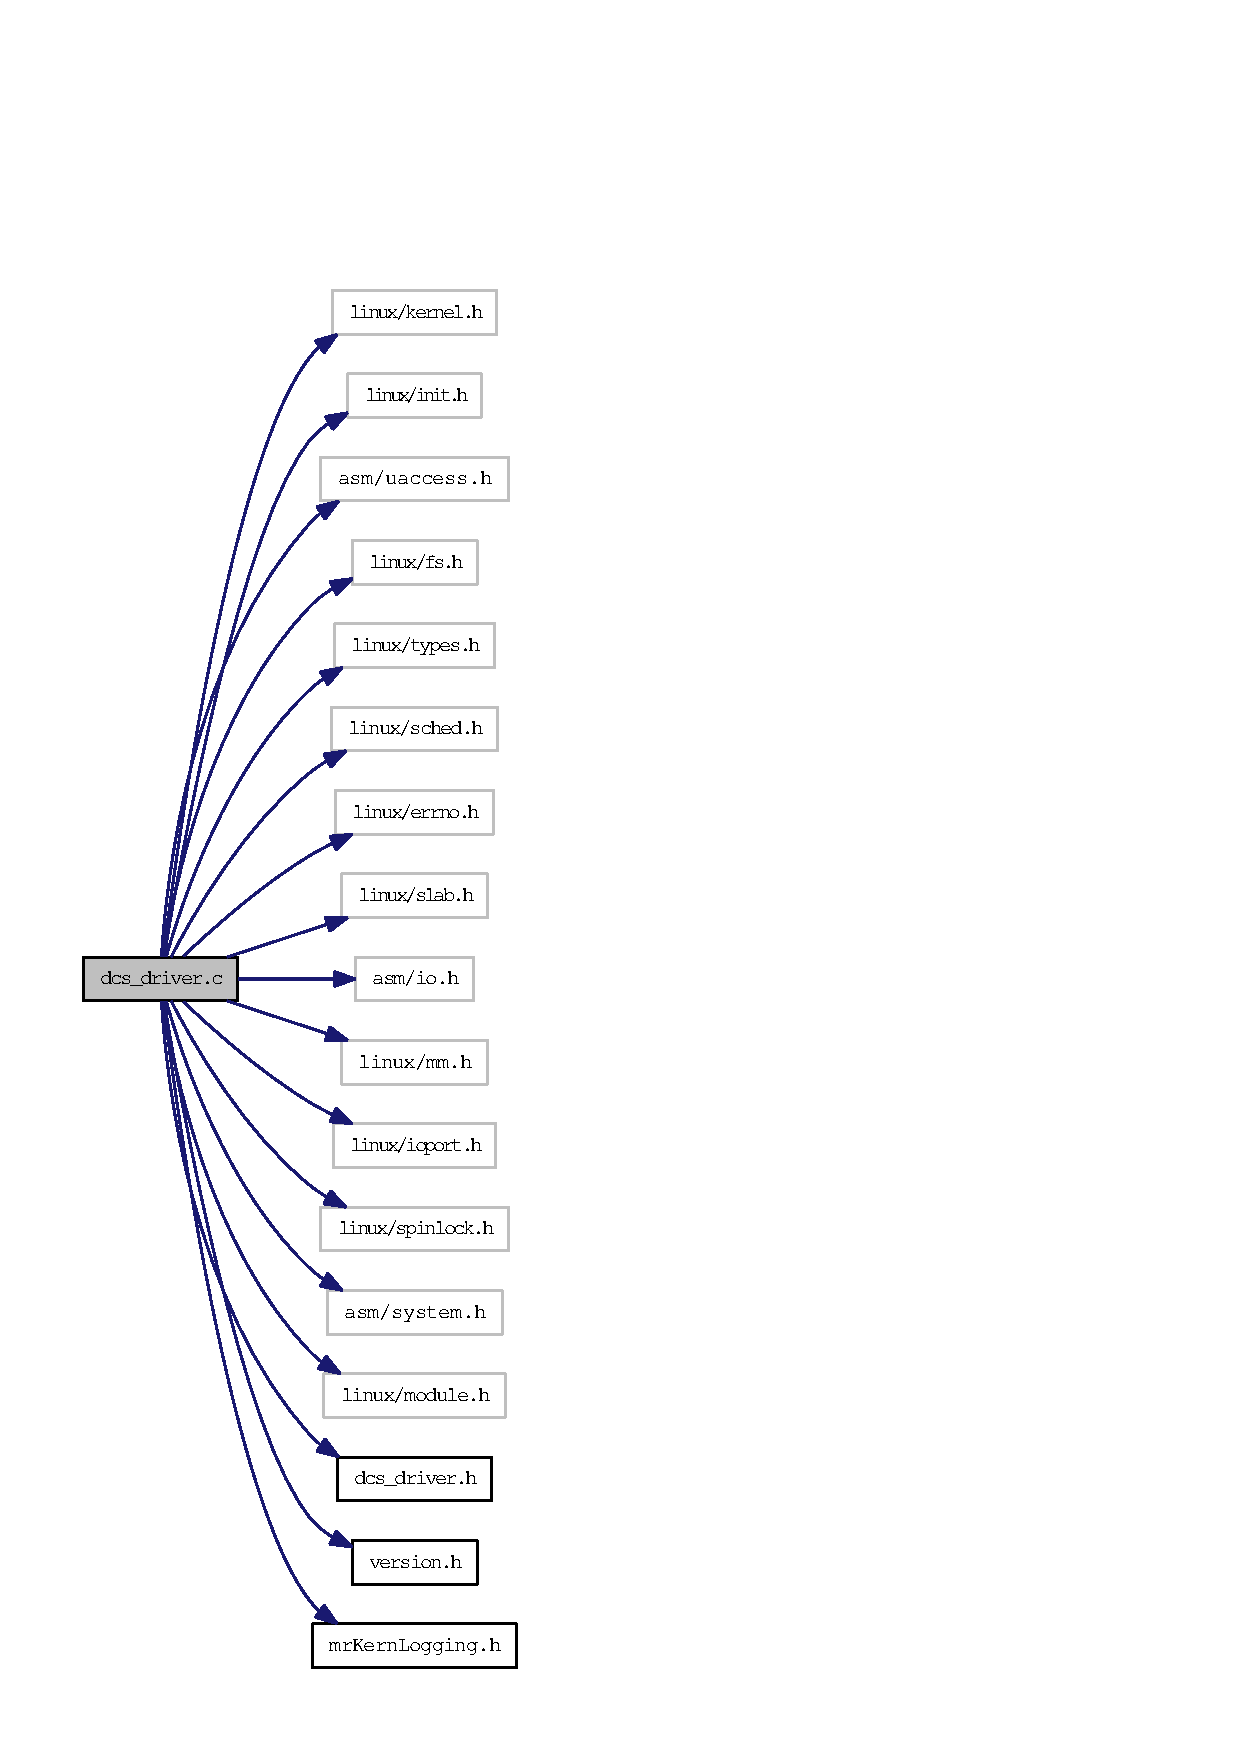
\includegraphics[width=126pt]{dcs__driver_8c__incl}
\end{center}
\end{figure}
\subsection*{Defines}
\begin{CompactItemize}
\item 
\#define \hyperlink{dcs__driver_8c_a7df9168b4a69449407f92158064f6c3}{DCSC\_\-TEST}
\end{CompactItemize}
\subsection*{Functions}
\begin{CompactItemize}
\item 
\hyperlink{dcs__driver_8c_ceea4740d376694aba7b9a9cc7678ea5}{module\_\-param} (\hyperlink{dcs__driver_8c_45c631d40e14d14a309abbe2b87ccd1b}{dcsc\_\-major\-ID}, int, S\_\-IRUSR$|$S\_\-IWUSR)
\item 
\hyperlink{dcs__driver_8c_0f08985cb950f96621515cfc98c5c4f8}{module\_\-param} (\hyperlink{dcs__driver_8c_9a8b5688625d4564010909cb4e23192f}{dcsc\_\-msgbuf\_\-in\_\-size}, int, S\_\-IRUSR$|$S\_\-IWUSR)
\item 
\hyperlink{dcs__driver_8c_e0c152bc8846983b45977e0f6da06524}{module\_\-param} (\hyperlink{dcs__driver_8c_57243357aaca143dc0a0e93dcd16eb89}{dcsc\_\-msgbuf\_\-out\_\-size}, int, S\_\-IRUSR$|$S\_\-IWUSR)
\item 
\hyperlink{dcs__driver_8c_172ae5ee71c938eb0332312d82619597}{module\_\-param} (\hyperlink{dcs__driver_8c_898ab396bb466832c0c38ecc37f16632}{dcsc\_\-regfile\_\-size}, int, S\_\-IRUSR$|$S\_\-IWUSR)
\item 
\hyperlink{dcs__driver_8c_b49852d26bb01c0e4a7addaf714bf8cf}{module\_\-param} (\hyperlink{dcs__driver_8c_03af36d4209f6364a9f7a5f1087f19f9}{msgbuf\_\-in\_\-physaddr}, uint, S\_\-IRUSR$|$S\_\-IWUSR)
\item 
\hyperlink{dcs__driver_8c_f217cc75a4e8cb0661b51a0bf23322fb}{module\_\-param} (\hyperlink{dcs__driver_8c_89c68fc835da1b91e1d93eecb77922b6}{msgbuf\_\-out\_\-physaddr}, uint, S\_\-IRUSR$|$S\_\-IWUSR)
\item 
\hyperlink{dcs__driver_8c_c6f3d27e211e849b579fac3c10ad3bf6}{module\_\-param} (\hyperlink{dcs__driver_8c_607a6fb1f19bf1e11ec4fa99dc7efecd}{regfile\_\-physaddr}, uint, S\_\-IRUSR$|$S\_\-IWUSR)
\item 
\hyperlink{dcs__driver_8c_53fff30413e173391c35bdc5481c1719}{MODULE\_\-AUTHOR} (\char`\"{}Matthias Richter\char`\"{})
\item 
\hyperlink{dcs__driver_8c_2eb38dffd9d03b7908c57b56ae9e9377}{MODULE\_\-DESCRIPTION} (\char`\"{}dcs-card register driver\char`\"{})
\item 
\hyperlink{dcs__driver_8c_d94b36675e7eb067ea3ce6ff9e244a44}{MODULE\_\-LICENSE} (\char`\"{}GPL\char`\"{})
\item 
static int \hyperlink{dcs__driver_8c_5fc9e61f41c571cca4373a64ca28d159}{memtest} (u32 begin, u32 size)
\item 
static int \hyperlink{dcs__driver_8c_24611c859ab5512627f0ebe5e71bb7df}{dcs\_\-comparevalue} (u32 begin, u32 size, u32 value)
\item 
static int \hyperlink{dcs__driver_8c_aec6947dd189feeedeb22af3fbc21d81}{dcs\_\-writevalue} (u32 begin, u32 size, u32 value)
\item 
static int \hyperlink{dcs__driver_8c_85874c4901b4b811c882944a3f77ff0e}{dcs\_\-read} (u32 begin, u32 size, u32 $\ast$buff)
\item 
static int \hyperlink{dcs__driver_8c_626a935595dad9fb4ce5cfdf4fd48f28}{dcs\_\-write} (u32 begin, u32 size, u32 $\ast$buff)
\item 
u32 \hyperlink{dcs__driver_8c_0f2edb55399fbd36008bbded20c5ecab}{find\-Buffer\-For\-Address} (loff\_\-t offset, int \hyperlink{dcs__driver_8c_269775bb092dfa3a11844c3d1883d988}{i\-Access\-Mode}, u32 $\ast$$\ast$pp\-Buffer, u32 $\ast$p\-Position, const char $\ast$$\ast$pp\-Buffer\-Name)
\item 
int \hyperlink{dcs__driver_8c_893d4c9fd97fbe478e6afc3f85688090}{Init\-Driver\-Lock} (void)
\item 
int \hyperlink{dcs__driver_8c_93880af66b0ace1e5b33443c98827142}{lock\-Activate} (void)
\item 
int \hyperlink{dcs__driver_8c_002955b4359e4c1406c3477aed9b3660}{lock\-Reset} (void)
\item 
int \hyperlink{dcs__driver_8c_4a2481d7c54d6ec0d99bc8716a8a021f}{check\-And\-Lock} (int i\-Seize\-Code, int pid)
\begin{CompactList}\small\item\em spin-lock protected check of the lock status variable. \item\end{CompactList}\item 
int \hyperlink{dcs__driver_8c_69f4b1ea76e4eeed7eb2fed3adc6e847}{lock\-Driver} (int i\-Seize\-Code, int i\-Time\-Out)
\begin{CompactList}\small\item\em Try to lock the driver, go to sleep if already locked. \item\end{CompactList}\item 
int \hyperlink{dcs__driver_8c_b24f1a24af4b992a55590712ef09fcc1}{unlock\-Driver} (void)
\begin{CompactList}\small\item\em Unlock the driver and wake up all sleeping processes. \item\end{CompactList}\item 
int \hyperlink{dcs__driver_8c_f65c837b7c30c1d6c4861e5dbb9a4e59}{seize\-Driver} (int i\-Seize\-Code)
\begin{CompactList}\small\item\em Lock the driver to a single application. \item\end{CompactList}\item 
int \hyperlink{dcs__driver_8c_6ccbabe02e6e0af40d2b653b2a158d40}{release\-Driver} (int i\-Seize\-Code)
\begin{CompactList}\small\item\em Release the driver which was locked to a single application. \item\end{CompactList}\item 
static loff\_\-t \hyperlink{dcs__driver_8c_1b18195d839987757d645e7761bdfbc1}{dcsc\_\-llseek} (struct file $\ast$filp, loff\_\-t off, int ref)
\item 
static int \hyperlink{dcs__driver_8c_8067a5efccbb89b363e4b12d4249bb07}{dcsc\_\-read} (struct file $\ast$filp, char $\ast$buf, size\_\-t count, loff\_\-t $\ast$f\_\-pos)
\item 
static int \hyperlink{dcs__driver_8c_0c28bf0d1a698b2c9c598715bd37a9cb}{dcsc\_\-write} (struct file $\ast$filp, const char $\ast$buf, size\_\-t count, loff\_\-t $\ast$f\_\-pos)
\item 
static int \hyperlink{dcs__driver_8c_1fc34702f88baf2a47a0434f6ea9e0cb}{dcsc\_\-open} (struct inode $\ast$inode, struct file $\ast$filp)
\item 
static int \hyperlink{dcs__driver_8c_5350bab3f3d6d1f1e2c84ecafa150d68}{dcsc\_\-close} (struct inode $\ast$inode, struct file $\ast$filp)
\item 
static int \hyperlink{dcs__driver_8c_c3b4c74273847bef0006306f638cc133}{dcsc\_\-mmap} (struct file $\ast$filp, struct vm\_\-area\_\-struct $\ast$vma)
\item 
static int \hyperlink{dcs__driver_8c_30d7523911ed6cebd68b1d5c34da9d64}{dcsc\_\-ioctl} (struct inode $\ast$inode, struct file $\ast$filp, unsigned int cmd, unsigned long arg)
\item 
void \hyperlink{dcs__driver_8c_4e947987f98c75955b980cb3f0990356}{cleanup\-Simulated\-Buffers} (void)
\item 
int \hyperlink{dcs__driver_8c_32eac9309c374d1bb41b744548b437b7}{init\-Simulated\-Buffers} (void)
\item 
int \hyperlink{dcs__driver_8c_e52690ce6969b799366b2c5feba67b8c}{init\_\-module} (void)
\item 
void \hyperlink{dcs__driver_8c_bb8e1606224e802418862b898888063a}{cleanup\_\-module} (void)
\end{CompactItemize}
\subsection*{Variables}
\begin{CompactItemize}
\item 
int \hyperlink{dcs__driver_8c_45c631d40e14d14a309abbe2b87ccd1b}{dcsc\_\-major\-ID} = 150
\item 
static int \hyperlink{dcs__driver_8c_9a8b5688625d4564010909cb4e23192f}{dcsc\_\-msgbuf\_\-in\_\-size} = 0x400
\item 
static int \hyperlink{dcs__driver_8c_57243357aaca143dc0a0e93dcd16eb89}{dcsc\_\-msgbuf\_\-out\_\-size} = 0x400
\item 
static int \hyperlink{dcs__driver_8c_898ab396bb466832c0c38ecc37f16632}{dcsc\_\-regfile\_\-size} = 0x10
\item 
static u32 $\ast$ \hyperlink{dcs__driver_8c_03af36d4209f6364a9f7a5f1087f19f9}{msgbuf\_\-in\_\-physaddr} = ((u32 $\ast$) 0x80000400)
\item 
static u32 $\ast$ \hyperlink{dcs__driver_8c_89c68fc835da1b91e1d93eecb77922b6}{msgbuf\_\-out\_\-physaddr} = ((u32 $\ast$) 0x80000800)
\item 
static u32 $\ast$ \hyperlink{dcs__driver_8c_607a6fb1f19bf1e11ec4fa99dc7efecd}{regfile\_\-physaddr} = ((u32 $\ast$) 0x80000060)
\item 
static u32 $\ast$ \hyperlink{dcs__driver_8c_a6f29aaef9f61f455e1eeb2890ca8300}{msgbuf\_\-in\_\-virtbase} = NULL
\item 
static u32 $\ast$ \hyperlink{dcs__driver_8c_6bd1f1592c9416c2bb4de131829a232d}{msgbuf\_\-out\_\-virtbase} = NULL
\item 
static u32 $\ast$ \hyperlink{dcs__driver_8c_dd264756338f180733724b4ea909d1cf}{regfile\_\-virtbase} = NULL
\item 
static char \hyperlink{dcs__driver_8c_cfec91dabccaee73c52b9ad0b8bbfd5c}{g\_\-logfilename} \mbox{[}LOG\_\-FILE\_\-NAME\_\-MAX\_\-LENGTH\mbox{]} = \char`\"{}\char`\"{}
\item 
static int \hyperlink{dcs__driver_8c_269775bb092dfa3a11844c3d1883d988}{i\-Access\-Mode} = ACCESS\_\-ALL
\item 
wait\_\-queue\_\-head\_\-t \hyperlink{dcs__driver_8c_c5ac2769997c4ac1e8307c4521c4b20e}{g\_\-wait\-Queue}
\item 
int \hyperlink{dcs__driver_8c_983d0af3572a91f1c34b942ff8954544}{g\_\-i\-Lock\-Reset} = 0
\item 
int \hyperlink{dcs__driver_8c_18b5596c6309017456c046d61b05e3b1}{g\_\-i\-Lock} = 0
\item 
int \hyperlink{dcs__driver_8c_750fd6e08c92777b860f11e575a4e804}{g\_\-i\-Lock\-Pid} = 0
\item 
int \hyperlink{dcs__driver_8c_2d3bbc70ca9389e34e840e3c3fade06d}{g\_\-i\-Seize\-Code} = 0
\item 
spinlock\_\-t \hyperlink{dcs__driver_8c_2f3f72c4a42056343b2c0ac401326cb4}{g\_\-spinlock}
\item 
int \hyperlink{dcs__driver_8c_c23aa679017a305c1a149016fea0c003}{g\_\-i\-Lock\-Initialized} = 0
\item 
file\_\-operations \hyperlink{dcs__driver_8c_010266ee96b0e2fd685de9f760d64dd8}{dcsc\_\-fops}
\end{CompactItemize}


\subsection{Define Documentation}
\hypertarget{dcs__driver_8c_a7df9168b4a69449407f92158064f6c3}{
\index{dcs_driver.c@{dcs\_\-driver.c}!DCSC_TEST@{DCSC\_\-TEST}}
\index{DCSC_TEST@{DCSC\_\-TEST}!dcs_driver.c@{dcs\_\-driver.c}}
\subsubsection[DCSC\_\-TEST]{\setlength{\rightskip}{0pt plus 5cm}\#define DCSC\_\-TEST}}
\label{dcs__driver_8c_a7df9168b4a69449407f92158064f6c3}




Definition at line 51 of file dcs\_\-driver.c.

Referenced by rcu\_\-flash\_\-read(), and rcu\_\-flash\_\-write().

\subsection{Function Documentation}
\hypertarget{dcs__driver_8c_4a2481d7c54d6ec0d99bc8716a8a021f}{
\index{dcs_driver.c@{dcs\_\-driver.c}!checkAndLock@{checkAndLock}}
\index{checkAndLock@{checkAndLock}!dcs_driver.c@{dcs\_\-driver.c}}
\subsubsection[checkAndLock]{\setlength{\rightskip}{0pt plus 5cm}int check\-And\-Lock (int {\em i\-Seize\-Code}, int {\em pid})}}
\label{dcs__driver_8c_4a2481d7c54d6ec0d99bc8716a8a021f}


spin-lock protected check of the lock status variable. 

If the lock is free it will be set. If the lock is owned by the current process the lock is incremented. The driver can be {\em master\/} locked by an application which causes the lock to return {\em permission denied\/} for requests by other applications. \begin{Desc}
\item[Parameters:]
\begin{description}
\item[{\em i\-Seize\-Code}]master lock code given by the application \item[{\em i\-Time\-Out}]time out (currently not used) \end{description}
\end{Desc}
\begin{Desc}
\item[Returns:]1 if free and now set, 0 if already blocked\par
 -ETIMEDOUT if time out\par
 -EPERM driver in master lock \end{Desc}


Definition at line 353 of file dcs\_\-driver.c.

References g\_\-i\-Lock, g\_\-i\-Lock\-Initialized, g\_\-i\-Lock\-Pid, g\_\-i\-Seize\-Code, g\_\-spinlock, LOG\_\-DBG, LOG\_\-DRIVER\_\-LCK, MR\_\-KERN\_\-DEBUG, and mrlogmessage().

Here is the call graph for this function:\begin{figure}[H]
\begin{center}
\leavevmode
\includegraphics[width=127pt]{dcs__driver_8c_4a2481d7c54d6ec0d99bc8716a8a021f_cgraph}
\end{center}
\end{figure}
\hypertarget{dcs__driver_8c_bb8e1606224e802418862b898888063a}{
\index{dcs_driver.c@{dcs\_\-driver.c}!cleanup_module@{cleanup\_\-module}}
\index{cleanup_module@{cleanup\_\-module}!dcs_driver.c@{dcs\_\-driver.c}}
\subsubsection[cleanup\_\-module]{\setlength{\rightskip}{0pt plus 5cm}void cleanup\_\-module (void)}}
\label{dcs__driver_8c_bb8e1606224e802418862b898888063a}




Definition at line 680 of file dcs\_\-driver.c.

References cleanup\-Real\-Buffers(), cleanup\-Simulated\-Buffers(), dcsc\_\-major\-ID, LOG\_\-INFO, and mrlogmessage().

Here is the call graph for this function:\begin{figure}[H]
\begin{center}
\leavevmode
\includegraphics[width=156pt]{dcs__driver_8c_bb8e1606224e802418862b898888063a_cgraph}
\end{center}
\end{figure}
\hypertarget{dcs__driver_8c_4e947987f98c75955b980cb3f0990356}{
\index{dcs_driver.c@{dcs\_\-driver.c}!cleanupSimulatedBuffers@{cleanupSimulatedBuffers}}
\index{cleanupSimulatedBuffers@{cleanupSimulatedBuffers}!dcs_driver.c@{dcs\_\-driver.c}}
\subsubsection[cleanupSimulatedBuffers]{\setlength{\rightskip}{0pt plus 5cm}void cleanup\-Simulated\-Buffers (void)}}
\label{dcs__driver_8c_4e947987f98c75955b980cb3f0990356}




Definition at line 591 of file dcs\_\-driver.c.

References msgbuf\_\-out\_\-virtbase, and regfile\_\-virtbase.

Referenced by cleanup\_\-module().\hypertarget{dcs__driver_8c_24611c859ab5512627f0ebe5e71bb7df}{
\index{dcs_driver.c@{dcs\_\-driver.c}!dcs_comparevalue@{dcs\_\-comparevalue}}
\index{dcs_comparevalue@{dcs\_\-comparevalue}!dcs_driver.c@{dcs\_\-driver.c}}
\subsubsection[dcs\_\-comparevalue]{\setlength{\rightskip}{0pt plus 5cm}static int dcs\_\-comparevalue (u32 {\em begin}, u32 {\em size}, u32 {\em value})\hspace{0.3cm}{\tt  \mbox{[}static\mbox{]}}}}
\label{dcs__driver_8c_24611c859ab5512627f0ebe5e71bb7df}




Definition at line 153 of file dcs\_\-driver.c.\hypertarget{dcs__driver_8c_85874c4901b4b811c882944a3f77ff0e}{
\index{dcs_driver.c@{dcs\_\-driver.c}!dcs_read@{dcs\_\-read}}
\index{dcs_read@{dcs\_\-read}!dcs_driver.c@{dcs\_\-driver.c}}
\subsubsection[dcs\_\-read]{\setlength{\rightskip}{0pt plus 5cm}static int dcs\_\-read (u32 {\em begin}, u32 {\em size}, u32 $\ast$ {\em buff})\hspace{0.3cm}{\tt  \mbox{[}static\mbox{]}}}}
\label{dcs__driver_8c_85874c4901b4b811c882944a3f77ff0e}




Definition at line 190 of file dcs\_\-driver.c.\hypertarget{dcs__driver_8c_626a935595dad9fb4ce5cfdf4fd48f28}{
\index{dcs_driver.c@{dcs\_\-driver.c}!dcs_write@{dcs\_\-write}}
\index{dcs_write@{dcs\_\-write}!dcs_driver.c@{dcs\_\-driver.c}}
\subsubsection[dcs\_\-write]{\setlength{\rightskip}{0pt plus 5cm}static int dcs\_\-write (u32 {\em begin}, u32 {\em size}, u32 $\ast$ {\em buff})\hspace{0.3cm}{\tt  \mbox{[}static\mbox{]}}}}
\label{dcs__driver_8c_626a935595dad9fb4ce5cfdf4fd48f28}




Definition at line 215 of file dcs\_\-driver.c.\hypertarget{dcs__driver_8c_aec6947dd189feeedeb22af3fbc21d81}{
\index{dcs_driver.c@{dcs\_\-driver.c}!dcs_writevalue@{dcs\_\-writevalue}}
\index{dcs_writevalue@{dcs\_\-writevalue}!dcs_driver.c@{dcs\_\-driver.c}}
\subsubsection[dcs\_\-writevalue]{\setlength{\rightskip}{0pt plus 5cm}static int dcs\_\-writevalue (u32 {\em begin}, u32 {\em size}, u32 {\em value})\hspace{0.3cm}{\tt  \mbox{[}static\mbox{]}}}}
\label{dcs__driver_8c_aec6947dd189feeedeb22af3fbc21d81}




Definition at line 168 of file dcs\_\-driver.c.\hypertarget{dcs__driver_8c_5350bab3f3d6d1f1e2c84ecafa150d68}{
\index{dcs_driver.c@{dcs\_\-driver.c}!dcsc_close@{dcsc\_\-close}}
\index{dcsc_close@{dcsc\_\-close}!dcs_driver.c@{dcs\_\-driver.c}}
\subsubsection[dcsc\_\-close]{\setlength{\rightskip}{0pt plus 5cm}static int dcsc\_\-close (struct inode $\ast$ {\em inode}, struct file $\ast$ {\em filp})\hspace{0.3cm}{\tt  \mbox{[}static\mbox{]}}}}
\label{dcs__driver_8c_5350bab3f3d6d1f1e2c84ecafa150d68}




Definition at line 871 of file dcs\_\-driver.c.

References LOG\_\-DBG, LOG\_\-OPEN\_\-CLOSE, MR\_\-KERN\_\-DEBUG, and mrlogmessage().

Here is the call graph for this function:\begin{figure}[H]
\begin{center}
\leavevmode
\includegraphics[width=119pt]{dcs__driver_8c_5350bab3f3d6d1f1e2c84ecafa150d68_cgraph}
\end{center}
\end{figure}
\hypertarget{dcs__driver_8c_30d7523911ed6cebd68b1d5c34da9d64}{
\index{dcs_driver.c@{dcs\_\-driver.c}!dcsc_ioctl@{dcsc\_\-ioctl}}
\index{dcsc_ioctl@{dcsc\_\-ioctl}!dcs_driver.c@{dcs\_\-driver.c}}
\subsubsection[dcsc\_\-ioctl]{\setlength{\rightskip}{0pt plus 5cm}static int dcsc\_\-ioctl (struct inode $\ast$ {\em inode}, struct file $\ast$ {\em filp}, unsigned int {\em cmd}, unsigned long {\em arg})\hspace{0.3cm}{\tt  \mbox{[}static\mbox{]}}}}
\label{dcs__driver_8c_30d7523911ed6cebd68b1d5c34da9d64}




Definition at line 885 of file dcs\_\-driver.c.

References dcsc\_\-msgbuf\_\-in\_\-size, dcsc\_\-msgbuf\_\-out\_\-size, dcsc\_\-regfile\_\-size, DRIVER\_\-MAJOR\_\-VERSION\_\-NUMBER, DRIVER\_\-MINOR\_\-VERSION\_\-NUMBER, g\_\-logfilename, g\_\-logflags, IOCTL\_\-ACTIVATE\_\-LOCK, IOCTL\_\-GET\_\-MSGBUF\_\-IN\_\-SIZE, IOCTL\_\-GET\_\-MSGBUF\_\-OUT\_\-SIZE, IOCTL\_\-GET\_\-REGFILE\_\-SIZE, IOCTL\_\-GET\_\-VERS\_\-STR\_\-SIZE, IOCTL\_\-GET\_\-VERSION, IOCTL\_\-GET\_\-VERSION\_\-V02, IOCTL\_\-LOCK\_\-DRIVER, IOCTL\_\-READ\_\-REG, IOCTL\_\-RELEASE\_\-DRIVER, IOCTL\_\-RESET\_\-LOCK, IOCTL\_\-SEIZE\_\-DRIVER, IOCTL\_\-SET\_\-DEBUG\_\-LEVEL, IOCTL\_\-SET\_\-LOG\_\-FILE, IOCTL\_\-TEST\_\-MSGBUF\_\-IN, IOCTL\_\-TEST\_\-MSGBUF\_\-OUT, IOCTL\_\-UNLOCK\_\-DRIVER, IOCTL\_\-WRITE\_\-REG, lock\-Activate(), lock\-Driver(), lock\-Reset(), LOG\_\-DBG, LOG\_\-ERROR, LOG\_\-INFO, LOG\_\-IOCTL, LOG\_\-WARNING, MR\_\-KERN\_\-DEBUG, mrlogmessage(), regfile\_\-virtbase, release\-Driver(), RELEASETYPE, seize\-Driver(), unlock\-Driver(), and VERSION\_\-STRING\_\-SIZE.

Here is the call graph for this function:\begin{figure}[H]
\begin{center}
\leavevmode
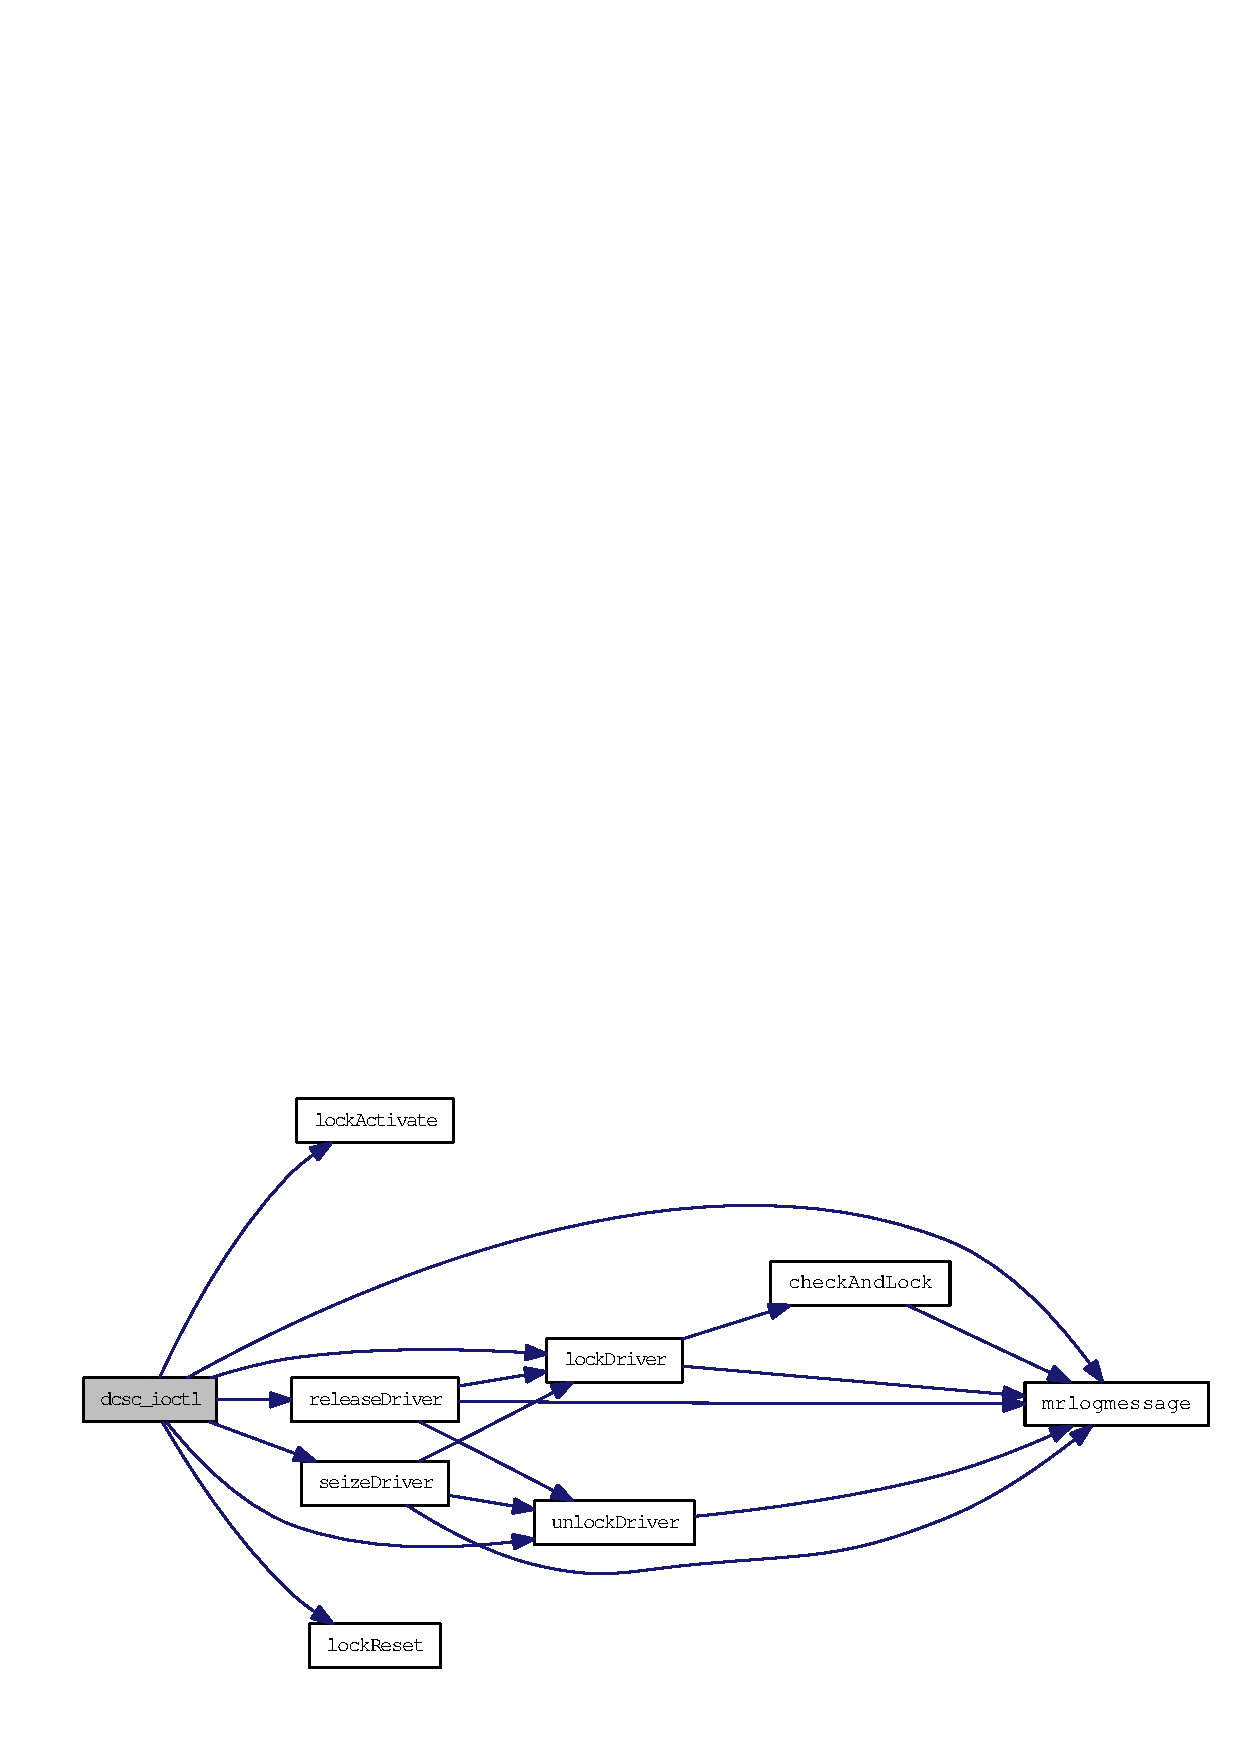
\includegraphics[width=292pt]{dcs__driver_8c_30d7523911ed6cebd68b1d5c34da9d64_cgraph}
\end{center}
\end{figure}
\hypertarget{dcs__driver_8c_1b18195d839987757d645e7761bdfbc1}{
\index{dcs_driver.c@{dcs\_\-driver.c}!dcsc_llseek@{dcsc\_\-llseek}}
\index{dcsc_llseek@{dcsc\_\-llseek}!dcs_driver.c@{dcs\_\-driver.c}}
\subsubsection[dcsc\_\-llseek]{\setlength{\rightskip}{0pt plus 5cm}static loff\_\-t dcsc\_\-llseek (struct file $\ast$ {\em filp}, loff\_\-t {\em off}, int {\em ref})\hspace{0.3cm}{\tt  \mbox{[}static\mbox{]}}}}
\label{dcs__driver_8c_1b18195d839987757d645e7761bdfbc1}




Definition at line 696 of file dcs\_\-driver.c.

References LOG\_\-DBG, LOG\_\-ERROR, LOG\_\-LLSEEK, MR\_\-KERN\_\-DEBUG, and mrlogmessage().

Here is the call graph for this function:\begin{figure}[H]
\begin{center}
\leavevmode
\includegraphics[width=120pt]{dcs__driver_8c_1b18195d839987757d645e7761bdfbc1_cgraph}
\end{center}
\end{figure}
\hypertarget{dcs__driver_8c_c3b4c74273847bef0006306f638cc133}{
\index{dcs_driver.c@{dcs\_\-driver.c}!dcsc_mmap@{dcsc\_\-mmap}}
\index{dcsc_mmap@{dcsc\_\-mmap}!dcs_driver.c@{dcs\_\-driver.c}}
\subsubsection[dcsc\_\-mmap]{\setlength{\rightskip}{0pt plus 5cm}static int dcsc\_\-mmap (struct file $\ast$ {\em filp}, struct vm\_\-area\_\-struct $\ast$ {\em vma})\hspace{0.3cm}{\tt  \mbox{[}static\mbox{]}}}}
\label{dcs__driver_8c_c3b4c74273847bef0006306f638cc133}




Definition at line 878 of file dcs\_\-driver.c.

References LOG\_\-DBG, LOG\_\-MMAP, MR\_\-KERN\_\-DEBUG, and mrlogmessage().

Here is the call graph for this function:\begin{figure}[H]
\begin{center}
\leavevmode
\includegraphics[width=122pt]{dcs__driver_8c_c3b4c74273847bef0006306f638cc133_cgraph}
\end{center}
\end{figure}
\hypertarget{dcs__driver_8c_1fc34702f88baf2a47a0434f6ea9e0cb}{
\index{dcs_driver.c@{dcs\_\-driver.c}!dcsc_open@{dcsc\_\-open}}
\index{dcsc_open@{dcsc\_\-open}!dcs_driver.c@{dcs\_\-driver.c}}
\subsubsection[dcsc\_\-open]{\setlength{\rightskip}{0pt plus 5cm}static int dcsc\_\-open (struct inode $\ast$ {\em inode}, struct file $\ast$ {\em filp})\hspace{0.3cm}{\tt  \mbox{[}static\mbox{]}}}}
\label{dcs__driver_8c_1fc34702f88baf2a47a0434f6ea9e0cb}




Definition at line 856 of file dcs\_\-driver.c.

References dcsc\_\-msgbuf\_\-in\_\-size, dcsc\_\-msgbuf\_\-out\_\-size, dcsc\_\-regfile\_\-size, LOG\_\-ERROR, LOG\_\-INFO, LOG\_\-OPEN\_\-CLOSE, MR\_\-KERN\_\-DEBUG, mrlogmessage(), msgbuf\_\-out\_\-virtbase, and regfile\_\-virtbase.

Here is the call graph for this function:\begin{figure}[H]
\begin{center}
\leavevmode
\includegraphics[width=119pt]{dcs__driver_8c_1fc34702f88baf2a47a0434f6ea9e0cb_cgraph}
\end{center}
\end{figure}
\hypertarget{dcs__driver_8c_8067a5efccbb89b363e4b12d4249bb07}{
\index{dcs_driver.c@{dcs\_\-driver.c}!dcsc_read@{dcsc\_\-read}}
\index{dcsc_read@{dcsc\_\-read}!dcs_driver.c@{dcs\_\-driver.c}}
\subsubsection[dcsc\_\-read]{\setlength{\rightskip}{0pt plus 5cm}static int dcsc\_\-read (struct file $\ast$ {\em filp}, char $\ast$ {\em buf}, size\_\-t {\em count}, loff\_\-t $\ast$ {\em f\_\-pos})\hspace{0.3cm}{\tt  \mbox{[}static\mbox{]}}}}
\label{dcs__driver_8c_8067a5efccbb89b363e4b12d4249bb07}




Definition at line 711 of file dcs\_\-driver.c.

References ACCESS\_\-ALL, dcs\_\-read(), dcsc\_\-msgbuf\_\-in\_\-size, dcsc\_\-msgbuf\_\-out\_\-size, dcsc\_\-regfile\_\-size, i\-Access\-Mode, LOG\_\-ERROR, LOG\_\-INFO, LOG\_\-READ\_\-WRITE, LOG\_\-WARNING, MR\_\-KERN\_\-DEBUG, mrlogmessage(), msgbuf\_\-out\_\-virtbase, and regfile\_\-virtbase.

Here is the call graph for this function:\begin{figure}[H]
\begin{center}
\leavevmode
\includegraphics[width=117pt]{dcs__driver_8c_8067a5efccbb89b363e4b12d4249bb07_cgraph}
\end{center}
\end{figure}
\hypertarget{dcs__driver_8c_0c28bf0d1a698b2c9c598715bd37a9cb}{
\index{dcs_driver.c@{dcs\_\-driver.c}!dcsc_write@{dcsc\_\-write}}
\index{dcsc_write@{dcsc\_\-write}!dcs_driver.c@{dcs\_\-driver.c}}
\subsubsection[dcsc\_\-write]{\setlength{\rightskip}{0pt plus 5cm}static int dcsc\_\-write (struct file $\ast$ {\em filp}, const char $\ast$ {\em buf}, size\_\-t {\em count}, loff\_\-t $\ast$ {\em f\_\-pos})\hspace{0.3cm}{\tt  \mbox{[}static\mbox{]}}}}
\label{dcs__driver_8c_0c28bf0d1a698b2c9c598715bd37a9cb}




Definition at line 786 of file dcs\_\-driver.c.

References ACCESS\_\-ALL, dcs\_\-write(), dcsc\_\-msgbuf\_\-in\_\-size, dcsc\_\-msgbuf\_\-out\_\-size, dcsc\_\-regfile\_\-size, i\-Access\-Mode, LOG\_\-ERROR, LOG\_\-INFO, LOG\_\-READ\_\-WRITE, LOG\_\-WARNING, MR\_\-KERN\_\-DEBUG, mrlogmessage(), msgbuf\_\-out\_\-virtbase, and regfile\_\-virtbase.

Here is the call graph for this function:\begin{figure}[H]
\begin{center}
\leavevmode
\includegraphics[width=118pt]{dcs__driver_8c_0c28bf0d1a698b2c9c598715bd37a9cb_cgraph}
\end{center}
\end{figure}
\hypertarget{dcs__driver_8c_0f2edb55399fbd36008bbded20c5ecab}{
\index{dcs_driver.c@{dcs\_\-driver.c}!findBufferForAddress@{findBufferForAddress}}
\index{findBufferForAddress@{findBufferForAddress}!dcs_driver.c@{dcs\_\-driver.c}}
\subsubsection[findBufferForAddress]{\setlength{\rightskip}{0pt plus 5cm}u32 find\-Buffer\-For\-Address (loff\_\-t {\em offset}, int {\em i\-Access\-Mode}, u32 $\ast$$\ast$ {\em pp\-Buffer}, u32 $\ast$ {\em p\-Position}, const char $\ast$$\ast$ {\em pp\-Buffer\-Name})}}
\label{dcs__driver_8c_0f2edb55399fbd36008bbded20c5ecab}




Definition at line 244 of file dcs\_\-driver.c.

References ACCESS\_\-IN\_\-BUFFER, ACCESS\_\-OUT\_\-BUFFER, ACCESS\_\-REGFILE, dcsc\_\-msgbuf\_\-in\_\-size, dcsc\_\-msgbuf\_\-out\_\-size, dcsc\_\-regfile\_\-size, LOG\_\-FLAG\_\-ALL, mrlogmessage(), msgbuf\_\-in\_\-virtbase, msgbuf\_\-out\_\-virtbase, and regfile\_\-virtbase.

Here is the call graph for this function:\begin{figure}[H]
\begin{center}
\leavevmode
\includegraphics[width=143pt]{dcs__driver_8c_0f2edb55399fbd36008bbded20c5ecab_cgraph}
\end{center}
\end{figure}
\hypertarget{dcs__driver_8c_e52690ce6969b799366b2c5feba67b8c}{
\index{dcs_driver.c@{dcs\_\-driver.c}!init_module@{init\_\-module}}
\index{init_module@{init\_\-module}!dcs_driver.c@{dcs\_\-driver.c}}
\subsubsection[init\_\-module]{\setlength{\rightskip}{0pt plus 5cm}int init\_\-module (void)}}
\label{dcs__driver_8c_e52690ce6969b799366b2c5feba67b8c}




Definition at line 645 of file dcs\_\-driver.c.

References dcsc\_\-fops, dcsc\_\-major\-ID, DRIVER\_\-MAJOR\_\-VERSION\_\-NUMBER, DRIVER\_\-MINOR\_\-VERSION\_\-NUMBER, Init\-Driver\-Lock(), init\-Real\-Buffers(), LOG\_\-ERROR, LOG\_\-INFO, mrlogmessage(), and RELEASETYPE.

Here is the call graph for this function:\begin{figure}[H]
\begin{center}
\leavevmode
\includegraphics[width=192pt]{dcs__driver_8c_e52690ce6969b799366b2c5feba67b8c_cgraph}
\end{center}
\end{figure}
\hypertarget{dcs__driver_8c_893d4c9fd97fbe478e6afc3f85688090}{
\index{dcs_driver.c@{dcs\_\-driver.c}!InitDriverLock@{InitDriverLock}}
\index{InitDriverLock@{InitDriverLock}!dcs_driver.c@{dcs\_\-driver.c}}
\subsubsection[InitDriverLock]{\setlength{\rightskip}{0pt plus 5cm}int Init\-Driver\-Lock (void)}}
\label{dcs__driver_8c_893d4c9fd97fbe478e6afc3f85688090}




Definition at line 308 of file dcs\_\-driver.c.

References g\_\-i\-Lock, g\_\-i\-Lock\-Initialized, g\_\-i\-Lock\-Pid, g\_\-i\-Lock\-Reset, g\_\-i\-Seize\-Code, g\_\-spinlock, and g\_\-wait\-Queue.\hypertarget{dcs__driver_8c_32eac9309c374d1bb41b744548b437b7}{
\index{dcs_driver.c@{dcs\_\-driver.c}!initSimulatedBuffers@{initSimulatedBuffers}}
\index{initSimulatedBuffers@{initSimulatedBuffers}!dcs_driver.c@{dcs\_\-driver.c}}
\subsubsection[initSimulatedBuffers]{\setlength{\rightskip}{0pt plus 5cm}int init\-Simulated\-Buffers (void)}}
\label{dcs__driver_8c_32eac9309c374d1bb41b744548b437b7}




Definition at line 601 of file dcs\_\-driver.c.

References dcs\_\-writevalue(), dcsc\_\-msgbuf\_\-in\_\-size, dcsc\_\-msgbuf\_\-out\_\-size, dcsc\_\-regfile\_\-size, LOG\_\-DBG, LOG\_\-ERROR, LOG\_\-INFO, LOG\_\-INTERNAL, memtest(), MR\_\-KERN\_\-DEBUG, mrlogmessage(), msgbuf\_\-out\_\-virtbase, and regfile\_\-virtbase.

Here is the call graph for this function:\begin{figure}[H]
\begin{center}
\leavevmode
\includegraphics[width=140pt]{dcs__driver_8c_32eac9309c374d1bb41b744548b437b7_cgraph}
\end{center}
\end{figure}
\hypertarget{dcs__driver_8c_93880af66b0ace1e5b33443c98827142}{
\index{dcs_driver.c@{dcs\_\-driver.c}!lockActivate@{lockActivate}}
\index{lockActivate@{lockActivate}!dcs_driver.c@{dcs\_\-driver.c}}
\subsubsection[lockActivate]{\setlength{\rightskip}{0pt plus 5cm}int lock\-Activate (void)}}
\label{dcs__driver_8c_93880af66b0ace1e5b33443c98827142}




Definition at line 321 of file dcs\_\-driver.c.

References g\_\-i\-Lock\-Reset.\hypertarget{dcs__driver_8c_69f4b1ea76e4eeed7eb2fed3adc6e847}{
\index{dcs_driver.c@{dcs\_\-driver.c}!lockDriver@{lockDriver}}
\index{lockDriver@{lockDriver}!dcs_driver.c@{dcs\_\-driver.c}}
\subsubsection[lockDriver]{\setlength{\rightskip}{0pt plus 5cm}int lock\-Driver (int {\em i\-Seize\-Code}, int {\em i\-Time\-Out})}}
\label{dcs__driver_8c_69f4b1ea76e4eeed7eb2fed3adc6e847}


Try to lock the driver, go to sleep if already locked. 

After the process got woken up it tries again to lock. \begin{Desc}
\item[Parameters:]
\begin{description}
\item[{\em i\-Seize\-Code}]master lock code given by the application \item[{\em i\-Time\-Out}]time out (currently not used) \end{description}
\end{Desc}
\begin{Desc}
\item[Returns:]1 if free and now set, 0 if already blocked\par
 -ETIMEDOUT if time out\par
 -EPERM driver in master lock \end{Desc}


Definition at line 382 of file dcs\_\-driver.c.

References check\-And\-Lock(), g\_\-i\-Lock\-Initialized, g\_\-i\-Lock\-Reset, g\_\-wait\-Queue, LOG\_\-DBG, LOG\_\-DRIVER\_\-LCK, MR\_\-KERN\_\-DEBUG, and mrlogmessage().

Here is the call graph for this function:\begin{figure}[H]
\begin{center}
\leavevmode
\includegraphics[width=178pt]{dcs__driver_8c_69f4b1ea76e4eeed7eb2fed3adc6e847_cgraph}
\end{center}
\end{figure}
\hypertarget{dcs__driver_8c_002955b4359e4c1406c3477aed9b3660}{
\index{dcs_driver.c@{dcs\_\-driver.c}!lockReset@{lockReset}}
\index{lockReset@{lockReset}!dcs_driver.c@{dcs\_\-driver.c}}
\subsubsection[lockReset]{\setlength{\rightskip}{0pt plus 5cm}int lock\-Reset (void)}}
\label{dcs__driver_8c_002955b4359e4c1406c3477aed9b3660}




Definition at line 328 of file dcs\_\-driver.c.

References g\_\-i\-Lock, g\_\-i\-Lock\-Initialized, g\_\-i\-Lock\-Pid, g\_\-i\-Lock\-Reset, g\_\-i\-Seize\-Code, and g\_\-wait\-Queue.\hypertarget{dcs__driver_8c_5fc9e61f41c571cca4373a64ca28d159}{
\index{dcs_driver.c@{dcs\_\-driver.c}!memtest@{memtest}}
\index{memtest@{memtest}!dcs_driver.c@{dcs\_\-driver.c}}
\subsubsection[memtest]{\setlength{\rightskip}{0pt plus 5cm}static int memtest (u32 {\em begin}, u32 {\em size})\hspace{0.3cm}{\tt  \mbox{[}static\mbox{]}}}}
\label{dcs__driver_8c_5fc9e61f41c571cca4373a64ca28d159}




Definition at line 131 of file dcs\_\-driver.c.\hypertarget{dcs__driver_8c_53fff30413e173391c35bdc5481c1719}{
\index{dcs_driver.c@{dcs\_\-driver.c}!MODULE_AUTHOR@{MODULE\_\-AUTHOR}}
\index{MODULE_AUTHOR@{MODULE\_\-AUTHOR}!dcs_driver.c@{dcs\_\-driver.c}}
\subsubsection[MODULE\_\-AUTHOR]{\setlength{\rightskip}{0pt plus 5cm}MODULE\_\-AUTHOR (\char`\"{}Matthias Richter\char`\"{})}}
\label{dcs__driver_8c_53fff30413e173391c35bdc5481c1719}


\hypertarget{dcs__driver_8c_2eb38dffd9d03b7908c57b56ae9e9377}{
\index{dcs_driver.c@{dcs\_\-driver.c}!MODULE_DESCRIPTION@{MODULE\_\-DESCRIPTION}}
\index{MODULE_DESCRIPTION@{MODULE\_\-DESCRIPTION}!dcs_driver.c@{dcs\_\-driver.c}}
\subsubsection[MODULE\_\-DESCRIPTION]{\setlength{\rightskip}{0pt plus 5cm}MODULE\_\-DESCRIPTION (\char`\"{}dcs-card register driver\char`\"{})}}
\label{dcs__driver_8c_2eb38dffd9d03b7908c57b56ae9e9377}


\hypertarget{dcs__driver_8c_d94b36675e7eb067ea3ce6ff9e244a44}{
\index{dcs_driver.c@{dcs\_\-driver.c}!MODULE_LICENSE@{MODULE\_\-LICENSE}}
\index{MODULE_LICENSE@{MODULE\_\-LICENSE}!dcs_driver.c@{dcs\_\-driver.c}}
\subsubsection[MODULE\_\-LICENSE]{\setlength{\rightskip}{0pt plus 5cm}MODULE\_\-LICENSE (\char`\"{}GPL\char`\"{})}}
\label{dcs__driver_8c_d94b36675e7eb067ea3ce6ff9e244a44}


\hypertarget{dcs__driver_8c_c6f3d27e211e849b579fac3c10ad3bf6}{
\index{dcs_driver.c@{dcs\_\-driver.c}!module_param@{module\_\-param}}
\index{module_param@{module\_\-param}!dcs_driver.c@{dcs\_\-driver.c}}
\subsubsection[module\_\-param]{\setlength{\rightskip}{0pt plus 5cm}module\_\-param (\hyperlink{dcs__driver_8c_607a6fb1f19bf1e11ec4fa99dc7efecd}{regfile\_\-physaddr}, uint, S\_\-IRUSR$|$ {\em S\_\-IWUSR})}}
\label{dcs__driver_8c_c6f3d27e211e849b579fac3c10ad3bf6}


\hypertarget{dcs__driver_8c_f217cc75a4e8cb0661b51a0bf23322fb}{
\index{dcs_driver.c@{dcs\_\-driver.c}!module_param@{module\_\-param}}
\index{module_param@{module\_\-param}!dcs_driver.c@{dcs\_\-driver.c}}
\subsubsection[module\_\-param]{\setlength{\rightskip}{0pt plus 5cm}module\_\-param (\hyperlink{dcs__driver_8c_89c68fc835da1b91e1d93eecb77922b6}{msgbuf\_\-out\_\-physaddr}, uint, S\_\-IRUSR$|$ {\em S\_\-IWUSR})}}
\label{dcs__driver_8c_f217cc75a4e8cb0661b51a0bf23322fb}


\hypertarget{dcs__driver_8c_b49852d26bb01c0e4a7addaf714bf8cf}{
\index{dcs_driver.c@{dcs\_\-driver.c}!module_param@{module\_\-param}}
\index{module_param@{module\_\-param}!dcs_driver.c@{dcs\_\-driver.c}}
\subsubsection[module\_\-param]{\setlength{\rightskip}{0pt plus 5cm}module\_\-param (\hyperlink{dcs__driver_8c_03af36d4209f6364a9f7a5f1087f19f9}{msgbuf\_\-in\_\-physaddr}, uint, S\_\-IRUSR$|$ {\em S\_\-IWUSR})}}
\label{dcs__driver_8c_b49852d26bb01c0e4a7addaf714bf8cf}


\hypertarget{dcs__driver_8c_172ae5ee71c938eb0332312d82619597}{
\index{dcs_driver.c@{dcs\_\-driver.c}!module_param@{module\_\-param}}
\index{module_param@{module\_\-param}!dcs_driver.c@{dcs\_\-driver.c}}
\subsubsection[module\_\-param]{\setlength{\rightskip}{0pt plus 5cm}module\_\-param (\hyperlink{dcs__driver_8c_898ab396bb466832c0c38ecc37f16632}{dcsc\_\-regfile\_\-size}, int, S\_\-IRUSR$|$ {\em S\_\-IWUSR})}}
\label{dcs__driver_8c_172ae5ee71c938eb0332312d82619597}


\hypertarget{dcs__driver_8c_e0c152bc8846983b45977e0f6da06524}{
\index{dcs_driver.c@{dcs\_\-driver.c}!module_param@{module\_\-param}}
\index{module_param@{module\_\-param}!dcs_driver.c@{dcs\_\-driver.c}}
\subsubsection[module\_\-param]{\setlength{\rightskip}{0pt plus 5cm}module\_\-param (\hyperlink{dcs__driver_8c_57243357aaca143dc0a0e93dcd16eb89}{dcsc\_\-msgbuf\_\-out\_\-size}, int, S\_\-IRUSR$|$ {\em S\_\-IWUSR})}}
\label{dcs__driver_8c_e0c152bc8846983b45977e0f6da06524}


\hypertarget{dcs__driver_8c_0f08985cb950f96621515cfc98c5c4f8}{
\index{dcs_driver.c@{dcs\_\-driver.c}!module_param@{module\_\-param}}
\index{module_param@{module\_\-param}!dcs_driver.c@{dcs\_\-driver.c}}
\subsubsection[module\_\-param]{\setlength{\rightskip}{0pt plus 5cm}module\_\-param (\hyperlink{dcs__driver_8c_9a8b5688625d4564010909cb4e23192f}{dcsc\_\-msgbuf\_\-in\_\-size}, int, S\_\-IRUSR$|$ {\em S\_\-IWUSR})}}
\label{dcs__driver_8c_0f08985cb950f96621515cfc98c5c4f8}


\hypertarget{dcs__driver_8c_ceea4740d376694aba7b9a9cc7678ea5}{
\index{dcs_driver.c@{dcs\_\-driver.c}!module_param@{module\_\-param}}
\index{module_param@{module\_\-param}!dcs_driver.c@{dcs\_\-driver.c}}
\subsubsection[module\_\-param]{\setlength{\rightskip}{0pt plus 5cm}module\_\-param (\hyperlink{dcs__driver_8c_45c631d40e14d14a309abbe2b87ccd1b}{dcsc\_\-major\-ID}, int, S\_\-IRUSR$|$ {\em S\_\-IWUSR})}}
\label{dcs__driver_8c_ceea4740d376694aba7b9a9cc7678ea5}


\hypertarget{dcs__driver_8c_6ccbabe02e6e0af40d2b653b2a158d40}{
\index{dcs_driver.c@{dcs\_\-driver.c}!releaseDriver@{releaseDriver}}
\index{releaseDriver@{releaseDriver}!dcs_driver.c@{dcs\_\-driver.c}}
\subsubsection[releaseDriver]{\setlength{\rightskip}{0pt plus 5cm}int release\-Driver (int {\em i\-Seize\-Code})}}
\label{dcs__driver_8c_6ccbabe02e6e0af40d2b653b2a158d40}


Release the driver which was locked to a single application. 

The is the pendant to \hyperlink{dcs__driver_8c_f65c837b7c30c1d6c4861e5dbb9a4e59}{seize\-Driver}. \begin{Desc}
\item[Parameters:]
\begin{description}
\item[{\em i\-Seize\-Code}]master lock code given by the application \end{description}
\end{Desc}
\begin{Desc}
\item[Returns:]$>$=0 if success, neg. error code if failed \end{Desc}


Definition at line 462 of file dcs\_\-driver.c.

References g\_\-i\-Seize\-Code, lock\-Driver(), LOG\_\-DRIVER\_\-LCK, LOG\_\-ERROR, LOG\_\-INFO, mrlogmessage(), and unlock\-Driver().

Here is the call graph for this function:\begin{figure}[H]
\begin{center}
\leavevmode
\includegraphics[width=236pt]{dcs__driver_8c_6ccbabe02e6e0af40d2b653b2a158d40_cgraph}
\end{center}
\end{figure}
\hypertarget{dcs__driver_8c_f65c837b7c30c1d6c4861e5dbb9a4e59}{
\index{dcs_driver.c@{dcs\_\-driver.c}!seizeDriver@{seizeDriver}}
\index{seizeDriver@{seizeDriver}!dcs_driver.c@{dcs\_\-driver.c}}
\subsubsection[seizeDriver]{\setlength{\rightskip}{0pt plus 5cm}int seize\-Driver (int {\em i\-Seize\-Code})}}
\label{dcs__driver_8c_f65c837b7c30c1d6c4861e5dbb9a4e59}


Lock the driver to a single application. 

The normal lock works for the different treads of that application, but no other application has the right to access. \begin{Desc}
\item[Parameters:]
\begin{description}
\item[{\em i\-Seize\-Code}]a code to identify the master application \end{description}
\end{Desc}
\begin{Desc}
\item[Returns:]$>$=0 if success, neg. error code if failed\par
 -EPERM driver seized by another application \end{Desc}


Definition at line 436 of file dcs\_\-driver.c.

References g\_\-i\-Seize\-Code, lock\-Driver(), LOG\_\-DRIVER\_\-LCK, LOG\_\-ERROR, LOG\_\-INFO, LOG\_\-WARNING, mrlogmessage(), and unlock\-Driver().

Here is the call graph for this function:\begin{figure}[H]
\begin{center}
\leavevmode
\includegraphics[width=232pt]{dcs__driver_8c_f65c837b7c30c1d6c4861e5dbb9a4e59_cgraph}
\end{center}
\end{figure}
\hypertarget{dcs__driver_8c_b24f1a24af4b992a55590712ef09fcc1}{
\index{dcs_driver.c@{dcs\_\-driver.c}!unlockDriver@{unlockDriver}}
\index{unlockDriver@{unlockDriver}!dcs_driver.c@{dcs\_\-driver.c}}
\subsubsection[unlockDriver]{\setlength{\rightskip}{0pt plus 5cm}int unlock\-Driver (void)}}
\label{dcs__driver_8c_b24f1a24af4b992a55590712ef09fcc1}


Unlock the driver and wake up all sleeping processes. 



Definition at line 403 of file dcs\_\-driver.c.

References g\_\-i\-Lock, g\_\-i\-Lock\-Initialized, g\_\-i\-Lock\-Pid, g\_\-spinlock, g\_\-wait\-Queue, LOG\_\-DBG, LOG\_\-DRIVER\_\-LCK, LOG\_\-ERROR, LOG\_\-WARNING, MR\_\-KERN\_\-DEBUG, and mrlogmessage().

Here is the call graph for this function:\begin{figure}[H]
\begin{center}
\leavevmode
\includegraphics[width=123pt]{dcs__driver_8c_b24f1a24af4b992a55590712ef09fcc1_cgraph}
\end{center}
\end{figure}


\subsection{Variable Documentation}
\hypertarget{dcs__driver_8c_010266ee96b0e2fd685de9f760d64dd8}{
\index{dcs_driver.c@{dcs\_\-driver.c}!dcsc_fops@{dcsc\_\-fops}}
\index{dcsc_fops@{dcsc\_\-fops}!dcs_driver.c@{dcs\_\-driver.c}}
\subsubsection[dcsc\_\-fops]{\setlength{\rightskip}{0pt plus 5cm}struct file\_\-operations \hyperlink{dcs__driver_8c_010266ee96b0e2fd685de9f760d64dd8}{dcsc\_\-fops}}}
\label{dcs__driver_8c_010266ee96b0e2fd685de9f760d64dd8}


\textbf{Initial value:}

\begin{Code}\begin{verbatim} {
  llseek:  dcsc_llseek,
  read:    dcsc_read,
  write:   dcsc_write,
  ioctl:   dcsc_ioctl,
  mmap:    dcsc_mmap,
  open:    dcsc_open,
  release: dcsc_close,
}
\end{verbatim}\end{Code}


Definition at line 501 of file dcs\_\-driver.c.\hypertarget{dcs__driver_8c_45c631d40e14d14a309abbe2b87ccd1b}{
\index{dcs_driver.c@{dcs\_\-driver.c}!dcsc_majorID@{dcsc\_\-majorID}}
\index{dcsc_majorID@{dcsc\_\-majorID}!dcs_driver.c@{dcs\_\-driver.c}}
\subsubsection[dcsc\_\-majorID]{\setlength{\rightskip}{0pt plus 5cm}int \hyperlink{dcs__driver_8c_45c631d40e14d14a309abbe2b87ccd1b}{dcsc\_\-major\-ID} = 150}}
\label{dcs__driver_8c_45c631d40e14d14a309abbe2b87ccd1b}




Definition at line 55 of file dcs\_\-driver.c.\hypertarget{dcs__driver_8c_9a8b5688625d4564010909cb4e23192f}{
\index{dcs_driver.c@{dcs\_\-driver.c}!dcsc_msgbuf_in_size@{dcsc\_\-msgbuf\_\-in\_\-size}}
\index{dcsc_msgbuf_in_size@{dcsc\_\-msgbuf\_\-in\_\-size}!dcs_driver.c@{dcs\_\-driver.c}}
\subsubsection[dcsc\_\-msgbuf\_\-in\_\-size]{\setlength{\rightskip}{0pt plus 5cm}int \hyperlink{dcs__driver_8c_9a8b5688625d4564010909cb4e23192f}{dcsc\_\-msgbuf\_\-in\_\-size} = 0x400\hspace{0.3cm}{\tt  \mbox{[}static\mbox{]}}}}
\label{dcs__driver_8c_9a8b5688625d4564010909cb4e23192f}




Definition at line 78 of file dcs\_\-driver.c.\hypertarget{dcs__driver_8c_57243357aaca143dc0a0e93dcd16eb89}{
\index{dcs_driver.c@{dcs\_\-driver.c}!dcsc_msgbuf_out_size@{dcsc\_\-msgbuf\_\-out\_\-size}}
\index{dcsc_msgbuf_out_size@{dcsc\_\-msgbuf\_\-out\_\-size}!dcs_driver.c@{dcs\_\-driver.c}}
\subsubsection[dcsc\_\-msgbuf\_\-out\_\-size]{\setlength{\rightskip}{0pt plus 5cm}int \hyperlink{dcs__driver_8c_57243357aaca143dc0a0e93dcd16eb89}{dcsc\_\-msgbuf\_\-out\_\-size} = 0x400\hspace{0.3cm}{\tt  \mbox{[}static\mbox{]}}}}
\label{dcs__driver_8c_57243357aaca143dc0a0e93dcd16eb89}




Definition at line 79 of file dcs\_\-driver.c.\hypertarget{dcs__driver_8c_898ab396bb466832c0c38ecc37f16632}{
\index{dcs_driver.c@{dcs\_\-driver.c}!dcsc_regfile_size@{dcsc\_\-regfile\_\-size}}
\index{dcsc_regfile_size@{dcsc\_\-regfile\_\-size}!dcs_driver.c@{dcs\_\-driver.c}}
\subsubsection[dcsc\_\-regfile\_\-size]{\setlength{\rightskip}{0pt plus 5cm}int \hyperlink{dcs__driver_8c_898ab396bb466832c0c38ecc37f16632}{dcsc\_\-regfile\_\-size} = 0x10\hspace{0.3cm}{\tt  \mbox{[}static\mbox{]}}}}
\label{dcs__driver_8c_898ab396bb466832c0c38ecc37f16632}




Definition at line 80 of file dcs\_\-driver.c.\hypertarget{dcs__driver_8c_18b5596c6309017456c046d61b05e3b1}{
\index{dcs_driver.c@{dcs\_\-driver.c}!g_iLock@{g\_\-iLock}}
\index{g_iLock@{g\_\-iLock}!dcs_driver.c@{dcs\_\-driver.c}}
\subsubsection[g\_\-iLock]{\setlength{\rightskip}{0pt plus 5cm}int \hyperlink{dcs__driver_8c_18b5596c6309017456c046d61b05e3b1}{g\_\-i\-Lock} = 0}}
\label{dcs__driver_8c_18b5596c6309017456c046d61b05e3b1}




Definition at line 302 of file dcs\_\-driver.c.\hypertarget{dcs__driver_8c_c23aa679017a305c1a149016fea0c003}{
\index{dcs_driver.c@{dcs\_\-driver.c}!g_iLockInitialized@{g\_\-iLockInitialized}}
\index{g_iLockInitialized@{g\_\-iLockInitialized}!dcs_driver.c@{dcs\_\-driver.c}}
\subsubsection[g\_\-iLockInitialized]{\setlength{\rightskip}{0pt plus 5cm}int \hyperlink{dcs__driver_8c_c23aa679017a305c1a149016fea0c003}{g\_\-i\-Lock\-Initialized} = 0}}
\label{dcs__driver_8c_c23aa679017a305c1a149016fea0c003}




Definition at line 306 of file dcs\_\-driver.c.\hypertarget{dcs__driver_8c_750fd6e08c92777b860f11e575a4e804}{
\index{dcs_driver.c@{dcs\_\-driver.c}!g_iLockPid@{g\_\-iLockPid}}
\index{g_iLockPid@{g\_\-iLockPid}!dcs_driver.c@{dcs\_\-driver.c}}
\subsubsection[g\_\-iLockPid]{\setlength{\rightskip}{0pt plus 5cm}int \hyperlink{dcs__driver_8c_750fd6e08c92777b860f11e575a4e804}{g\_\-i\-Lock\-Pid} = 0}}
\label{dcs__driver_8c_750fd6e08c92777b860f11e575a4e804}




Definition at line 303 of file dcs\_\-driver.c.\hypertarget{dcs__driver_8c_983d0af3572a91f1c34b942ff8954544}{
\index{dcs_driver.c@{dcs\_\-driver.c}!g_iLockReset@{g\_\-iLockReset}}
\index{g_iLockReset@{g\_\-iLockReset}!dcs_driver.c@{dcs\_\-driver.c}}
\subsubsection[g\_\-iLockReset]{\setlength{\rightskip}{0pt plus 5cm}int \hyperlink{dcs__driver_8c_983d0af3572a91f1c34b942ff8954544}{g\_\-i\-Lock\-Reset} = 0}}
\label{dcs__driver_8c_983d0af3572a91f1c34b942ff8954544}




Definition at line 301 of file dcs\_\-driver.c.\hypertarget{dcs__driver_8c_2d3bbc70ca9389e34e840e3c3fade06d}{
\index{dcs_driver.c@{dcs\_\-driver.c}!g_iSeizeCode@{g\_\-iSeizeCode}}
\index{g_iSeizeCode@{g\_\-iSeizeCode}!dcs_driver.c@{dcs\_\-driver.c}}
\subsubsection[g\_\-iSeizeCode]{\setlength{\rightskip}{0pt plus 5cm}int \hyperlink{dcs__driver_8c_2d3bbc70ca9389e34e840e3c3fade06d}{g\_\-i\-Seize\-Code} = 0}}
\label{dcs__driver_8c_2d3bbc70ca9389e34e840e3c3fade06d}




Definition at line 304 of file dcs\_\-driver.c.\hypertarget{dcs__driver_8c_cfec91dabccaee73c52b9ad0b8bbfd5c}{
\index{dcs_driver.c@{dcs\_\-driver.c}!g_logfilename@{g\_\-logfilename}}
\index{g_logfilename@{g\_\-logfilename}!dcs_driver.c@{dcs\_\-driver.c}}
\subsubsection[g\_\-logfilename]{\setlength{\rightskip}{0pt plus 5cm}char \hyperlink{dcs__driver_8c_cfec91dabccaee73c52b9ad0b8bbfd5c}{g\_\-logfilename}\mbox{[}LOG\_\-FILE\_\-NAME\_\-MAX\_\-LENGTH\mbox{]} = \char`\"{}\char`\"{}\hspace{0.3cm}{\tt  \mbox{[}static\mbox{]}}}}
\label{dcs__driver_8c_cfec91dabccaee73c52b9ad0b8bbfd5c}




Definition at line 90 of file dcs\_\-driver.c.\hypertarget{dcs__driver_8c_2f3f72c4a42056343b2c0ac401326cb4}{
\index{dcs_driver.c@{dcs\_\-driver.c}!g_spinlock@{g\_\-spinlock}}
\index{g_spinlock@{g\_\-spinlock}!dcs_driver.c@{dcs\_\-driver.c}}
\subsubsection[g\_\-spinlock]{\setlength{\rightskip}{0pt plus 5cm}spinlock\_\-t \hyperlink{dcs__driver_8c_2f3f72c4a42056343b2c0ac401326cb4}{g\_\-spinlock}}}
\label{dcs__driver_8c_2f3f72c4a42056343b2c0ac401326cb4}




Definition at line 305 of file dcs\_\-driver.c.\hypertarget{dcs__driver_8c_c5ac2769997c4ac1e8307c4521c4b20e}{
\index{dcs_driver.c@{dcs\_\-driver.c}!g_waitQueue@{g\_\-waitQueue}}
\index{g_waitQueue@{g\_\-waitQueue}!dcs_driver.c@{dcs\_\-driver.c}}
\subsubsection[g\_\-waitQueue]{\setlength{\rightskip}{0pt plus 5cm}wait\_\-queue\_\-head\_\-t \hyperlink{dcs__driver_8c_c5ac2769997c4ac1e8307c4521c4b20e}{g\_\-wait\-Queue}}}
\label{dcs__driver_8c_c5ac2769997c4ac1e8307c4521c4b20e}




Definition at line 300 of file dcs\_\-driver.c.\hypertarget{dcs__driver_8c_269775bb092dfa3a11844c3d1883d988}{
\index{dcs_driver.c@{dcs\_\-driver.c}!iAccessMode@{iAccessMode}}
\index{iAccessMode@{iAccessMode}!dcs_driver.c@{dcs\_\-driver.c}}
\subsubsection[iAccessMode]{\setlength{\rightskip}{0pt plus 5cm}int \hyperlink{dcs__driver_8c_269775bb092dfa3a11844c3d1883d988}{i\-Access\-Mode} = ACCESS\_\-ALL\hspace{0.3cm}{\tt  \mbox{[}static\mbox{]}}}}
\label{dcs__driver_8c_269775bb092dfa3a11844c3d1883d988}




Definition at line 120 of file dcs\_\-driver.c.\hypertarget{dcs__driver_8c_03af36d4209f6364a9f7a5f1087f19f9}{
\index{dcs_driver.c@{dcs\_\-driver.c}!msgbuf_in_physaddr@{msgbuf\_\-in\_\-physaddr}}
\index{msgbuf_in_physaddr@{msgbuf\_\-in\_\-physaddr}!dcs_driver.c@{dcs\_\-driver.c}}
\subsubsection[msgbuf\_\-in\_\-physaddr]{\setlength{\rightskip}{0pt plus 5cm}u32$\ast$ \hyperlink{dcs__driver_8c_03af36d4209f6364a9f7a5f1087f19f9}{msgbuf\_\-in\_\-physaddr} = ((u32 $\ast$) 0x80000400)\hspace{0.3cm}{\tt  \mbox{[}static\mbox{]}}}}
\label{dcs__driver_8c_03af36d4209f6364a9f7a5f1087f19f9}




Definition at line 81 of file dcs\_\-driver.c.\hypertarget{dcs__driver_8c_a6f29aaef9f61f455e1eeb2890ca8300}{
\index{dcs_driver.c@{dcs\_\-driver.c}!msgbuf_in_virtbase@{msgbuf\_\-in\_\-virtbase}}
\index{msgbuf_in_virtbase@{msgbuf\_\-in\_\-virtbase}!dcs_driver.c@{dcs\_\-driver.c}}
\subsubsection[msgbuf\_\-in\_\-virtbase]{\setlength{\rightskip}{0pt plus 5cm}u32$\ast$ \hyperlink{dcs__driver_8c_a6f29aaef9f61f455e1eeb2890ca8300}{msgbuf\_\-in\_\-virtbase} = NULL\hspace{0.3cm}{\tt  \mbox{[}static\mbox{]}}}}
\label{dcs__driver_8c_a6f29aaef9f61f455e1eeb2890ca8300}




Definition at line 86 of file dcs\_\-driver.c.\hypertarget{dcs__driver_8c_89c68fc835da1b91e1d93eecb77922b6}{
\index{dcs_driver.c@{dcs\_\-driver.c}!msgbuf_out_physaddr@{msgbuf\_\-out\_\-physaddr}}
\index{msgbuf_out_physaddr@{msgbuf\_\-out\_\-physaddr}!dcs_driver.c@{dcs\_\-driver.c}}
\subsubsection[msgbuf\_\-out\_\-physaddr]{\setlength{\rightskip}{0pt plus 5cm}u32$\ast$ \hyperlink{dcs__driver_8c_89c68fc835da1b91e1d93eecb77922b6}{msgbuf\_\-out\_\-physaddr} = ((u32 $\ast$) 0x80000800)\hspace{0.3cm}{\tt  \mbox{[}static\mbox{]}}}}
\label{dcs__driver_8c_89c68fc835da1b91e1d93eecb77922b6}




Definition at line 82 of file dcs\_\-driver.c.\hypertarget{dcs__driver_8c_6bd1f1592c9416c2bb4de131829a232d}{
\index{dcs_driver.c@{dcs\_\-driver.c}!msgbuf_out_virtbase@{msgbuf\_\-out\_\-virtbase}}
\index{msgbuf_out_virtbase@{msgbuf\_\-out\_\-virtbase}!dcs_driver.c@{dcs\_\-driver.c}}
\subsubsection[msgbuf\_\-out\_\-virtbase]{\setlength{\rightskip}{0pt plus 5cm}u32$\ast$ \hyperlink{dcs__driver_8c_6bd1f1592c9416c2bb4de131829a232d}{msgbuf\_\-out\_\-virtbase} = NULL\hspace{0.3cm}{\tt  \mbox{[}static\mbox{]}}}}
\label{dcs__driver_8c_6bd1f1592c9416c2bb4de131829a232d}




Definition at line 87 of file dcs\_\-driver.c.\hypertarget{dcs__driver_8c_607a6fb1f19bf1e11ec4fa99dc7efecd}{
\index{dcs_driver.c@{dcs\_\-driver.c}!regfile_physaddr@{regfile\_\-physaddr}}
\index{regfile_physaddr@{regfile\_\-physaddr}!dcs_driver.c@{dcs\_\-driver.c}}
\subsubsection[regfile\_\-physaddr]{\setlength{\rightskip}{0pt plus 5cm}u32$\ast$ \hyperlink{dcs__driver_8c_607a6fb1f19bf1e11ec4fa99dc7efecd}{regfile\_\-physaddr} = ((u32 $\ast$) 0x80000060)\hspace{0.3cm}{\tt  \mbox{[}static\mbox{]}}}}
\label{dcs__driver_8c_607a6fb1f19bf1e11ec4fa99dc7efecd}




Definition at line 83 of file dcs\_\-driver.c.\hypertarget{dcs__driver_8c_dd264756338f180733724b4ea909d1cf}{
\index{dcs_driver.c@{dcs\_\-driver.c}!regfile_virtbase@{regfile\_\-virtbase}}
\index{regfile_virtbase@{regfile\_\-virtbase}!dcs_driver.c@{dcs\_\-driver.c}}
\subsubsection[regfile\_\-virtbase]{\setlength{\rightskip}{0pt plus 5cm}u32$\ast$ \hyperlink{dcs__driver_8c_dd264756338f180733724b4ea909d1cf}{regfile\_\-virtbase} = NULL\hspace{0.3cm}{\tt  \mbox{[}static\mbox{]}}}}
\label{dcs__driver_8c_dd264756338f180733724b4ea909d1cf}




Definition at line 88 of file dcs\_\-driver.c.